% siminos/spatiotemp/chapter/examSawtoothLin.tex
% $Author: predrag $ $Date: 2019-12-18 14:16:20 -0500 (Wed, 18 Dec 2019) $


%%% input by % siminos/spatiotemp/chapter/catMap.tex %%%%%
%\section{Any piecewise linear map has ``linear code''}
%\label{exam:tentMapSymbDyn}

%%%%%%%%%%%%%%%%%%%%%%%%%%%%%%%%%%%%%%%%%%%%%%%%%%%%%%%%%%%%%%%%%%
%\FIG{
\begin{figure}
  \centering
{(a)}
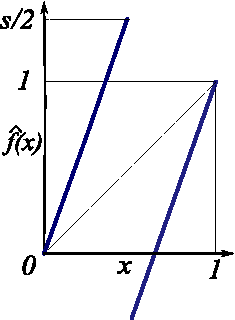
\includegraphics[width=0.36\textwidth]{fig_d_1CL18}
~~~
{(b)}
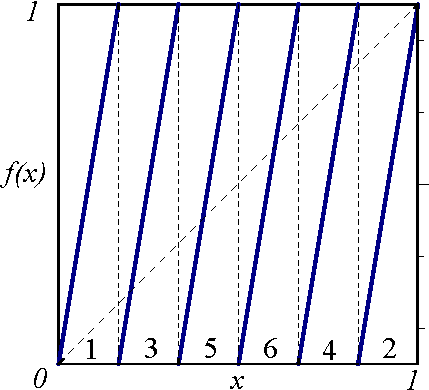
\includegraphics[width=0.32\textwidth]{fig_d_2}
  \caption{\label{fig-d-1}
(a) $\hflow{}{\hx}$, the full space sawtooth map \refeq{KD-map}, $\ExpaEig >
2$.
(b) $\flow{}{x}$, the sawtooth map restricted to the unit circle
\refeq{circ-m}, $\ExpaEig=6$.
            }
\end{figure}
%%%%%%%%%%%%%%%%%%%%%%%%%%%%%%%%%%%%%%%%%%%%%%%%%%%%%%%%%%%%%%%%%%
%
%%%%%%%%%%%%%%%%%%%%%%%%%%%%%%%%%%%%%%%%%%%%%%%%%%%%%%%
\example{Linear code for a piecewise linear map.}{\label{exam:SawtoothLin}
the piecewise linear map of \reffig{fig-d-1}
        \jumpBack{exam:SawtoothLin}
    } % end \example{exam:SawtoothLin}
%%%%%%%%%%%%%%%%%%%%%%%%%%%%%%%%%%%%%%%%%%%%%%%%%%%%%%%
